\documentclass[10pt]{article}
\usepackage[a4paper, total={170mm, 257mm}]{geometry}

\usepackage[
backend=biber,
style=nature,
sorting=none
]{biblatex}
\addbibresource{References.bib}
%\bibliographystyle{unsrt}


\usepackage{amsmath}
\usepackage{amssymb}
\usepackage{upgreek}
\usepackage{dsfont}
\usepackage{esint} % various fancy integral symbols
\usepackage{mathrsfs} % for \mathscr

% fancy notation stuff
\usepackage{accents}
% vector arrows under the symbol to distinguish covariant and contravariant
\newcommand\undervec[1]{\underaccent{\vec}{#1}}

\usepackage{siunitx}
\DeclareSIUnit{\litre}{l} % litres as lower case l (upper case L by default)

%\usepackage{hyperref}

\usepackage{graphicx} % Required for inserting images
\usepackage{multicol}
\usepackage{mathpazo}
\usepackage[font=sf,labelfont=bf]{caption}

% title, headings, abstract heading in sans serif font and maybe color
%\usepackage{sectsty}
%\usepackage{titling}
%\usepackage[sf,bf,pagestyles]{titlesec}
\usepackage[dvipsnames]{xcolor}
\usepackage{sectsty}
\usepackage{abstract}
\renewcommand\abstractnamefont{\sffamily\bfseries}%\color{Maroon}}
%\chapterfont{\color{blue}}  % sets colour of chapters
\sectionfont{\sffamily}%\color{Maroon}}  % sets colour of sections
\subsectionfont{\sffamily}%\color{Maroon}}  % sets colour of subsections
\subsubsectionfont{\sffamily}  % sets colour of subsections





% TO DO's
\newcommand{\todo}[1]{ {\color{ForestGreen} [#1]} }

\graphicspath{{figures/}}

\usepackage{lipsum} 

% referencing commands
\newcommand{\seefig}[2]{\mbox{\sffamily($\rightarrow$ Fig. \ref{#1}#2)}}
\newcommand{\reffig}[2]{\mbox{\sffamily{Figure \ref{#1}#2}}}


\title{\sffamily\bfseries\color{Maroon} Fourier Plane Scattering Spectroscopy\\of Plasmonic Janus Particles}
\author{Felix H. Patzschke, A. Markus Anton and *Frank Cichos}
%\date{November 2023}
\date{}



\begin{document}
%\allsectionsfont{\sffamily}

\maketitle

\begin{abstract}\sffamily \vspace{-1em} 
%The light-matter interactions of plasmonic nanostructures are of great importance to [whom?].
%For plasmonic Janus particles in particular, which are established as an often-used tool in active matter research, the [???] is two-fold. [...]
%Metal-coated Janus particles have established themselves as a valuable tool in active matter research \cite{MONA-flow-fields} and related fields, owing to their plasmonically active nanostructures which allow for both excellent visibility in dark-field applications, as well as for efficient heating and, consequently, motility. \cite{MONA-thermotaxis, MONA-photon-nudging-1} 
%With light-matter interactions enhanced through their plasmonically active nanostructures, metal-coated Janus particles allow for both excellent visibility in dark-field applications as well as efficient heating and, consequently, motility \cite{MONA-thermotaxis, MONA-photon-nudging-1}, making them a valuable tool for active matter research. \cite{MONA-flow-fields}
%In recent years, theoretical predictions have been made of counter-intuitive optically enabled behaviours of such particles. \cite{Ilic2017}
%Nonetheless, these light-matter interactions are not yet thoroughly understood; in particular, there does not yet exist a proven method of inferring the out-of-image-plane orientation of a spherical Janus particle from its dark-field image. 
%Nonetheless, these light-matter interactions are not yet thoroughly understood.

%We present an experimental method for the orientation-dependent scattering spectroscopy of such anisotropic microscale particles. 
% $\SI{1}{\micro\meter}$ PS + $\SI{50}{\nano\meter}$ Au
%We analysed the scattering behaviour of \mbox{1µm PS + 50 nm Au} Janus Particles, resolving for wavelength, direction of illumination and scattering angle.
%under dark-field illumination and reproduced the results by finite-elements simulations. 
%We find well-discernible spectral features, particularly in the NIR range, that appear or disappear, depending on the orientation of the JP. 
%Further, we reproduced the experimental results by finite-element simulations.
%These findings may be worked into a method of determining the notoriously elusive out-of-plane orientation of spherical JPs, possibly even in real-time.

%We identify spectral markers, particularly in the near infrared range, that depend heavily on the orientation of the Janus particle; a result that may enable a new method of determining the notoriously elusive [to do: reference] out-of-plane orientation of spherical JPs, possibly even in real-time.
Plasmonic Janus particles consist of dielectric core particles with a thin metallic cap on one side and are widely used in active matter research. \cite{MONA-flow-fields} 
The plasmonic cap enhances optical scattering and absorption, allowing for self-propulsion through temperature gradients as well as efficient trapping and tracking. \cite{MONA-thermotaxis, MONA-photon-nudging-1} 
The asymmetry of such a particle gives rise to surface plasmon modes whose excitation is sensitive to the angle at which the particle is illuminated. 
Even though the angle of illumination strongly influences the particle's scattering response, the optical properties of such metallic caps have hardly been investigated. 

We probe the light scattering of individual micrometre-sized, spherical, Au-coated Janus particles by means of Selective Illumination Multiplexed Fourier Plane Spectroscopy. 
This novel method allows us to explore microparticles' scattering characteristics resolved for wavelength, angle of illumination and scattering angle. 

In addition, we supplement our experimental results with finite-element simulations and correlate spectral markers to orientation-dependent surface plasmon modes. 
This additional information on the correlation of angular and spectral information could pave the way for new methods of orientation detection. They also shed new light on the interaction of such spherically capped particles with light inducing forces and torques. \cite{Ilic2017, BA}
 \\ \end{abstract}





\section*{Key Message}

\subsection*{Motivation}
We consider JPs with a plasmonically active cap. 
The \textbf{light-matter interaction} of the cap is 
\begin{itemize}
    \item \textbf{interesting:} 
    Enhanced absorption leads to heating.
    Together with the anisotropy of the particle, it leads to directed propulsion.
    Enhanced scattering leads to good visibility in imaging (tracking etc.).
    Propulsion and tracking leads to usefulness in active matter research. 
    \item \textbf{non-trivial:}
    Particle size and wavelength are roughly equal, therefore there are no easy approximations to describe the interaction (ray optics for large particle, dipole for small particle).
    Anisotropy of the particle leads to orientation-dependence of the light-matter interaction. 

    Some purely numerical studies suggest that a linearly polarized light field can transfer angular momentum in a really weird way. 
\end{itemize}

To our knowledge, this light-matter interaction has not yet been systematically studied. 
Orientation-dependent scattering studies of plasmonic nanostructures\footnote{specifically Au nano-rods and -triangles, sized between 100 and 150 nm} \emph{have} been performed, \cite{Islam2021} but with a limited capability for spectral resolution\footnote{literally just RGB}. 
Also, the angular distribution of the scattered light was entirely neglected. 
\\ 

This was a valid mode of operation for the particles they worked with all of which were smaller than any wavelength considered. 
But if the particles of interest are approximately the same size as the wavelengths considered, ...? 

\subsection*{Theory of scattering}
We have a good point of comparison in Mie theory: 
It models the LMI for particles on this very same length scale, provided they are maximally symmetric. 
Here, light is scattered in all kinds of directions at different intensities.

\subsection*{We present a new experimental method}
In order to measure the dependence of the scattering intensity on wavelength, direction of illumination and scattering angle, \textbf{we devised this experimental procedure:}

\textbf{Selective Illumination Multiplexed Fourier Plane Spectroscopy}
\begin{figure*}[h!]
    \centering
    \includegraphics[width=\textwidth]{[fig] setup (placeholder).jpg}
    \caption{(Placeholder) 
    {\sffamily\bfseries A:} Schematics of all apertures in the optical path. 
    {\sffamily\bfseries C:} Schematic of the imaging optics. 
    {\sffamily\bfseries D:} The virtually constant refractive index in the region surrounding the particle under observation. 
    {\sffamily\bfseries E:} Parameters describing the orientation of the system.
    }
    \label{fig:setup}
\end{figure*}

It's a combination of dark-field microscopy, Fourier plane imaging, confocal imaging and visible light spectroscopy. 
\begin{figure*}[h!]
    \centering
    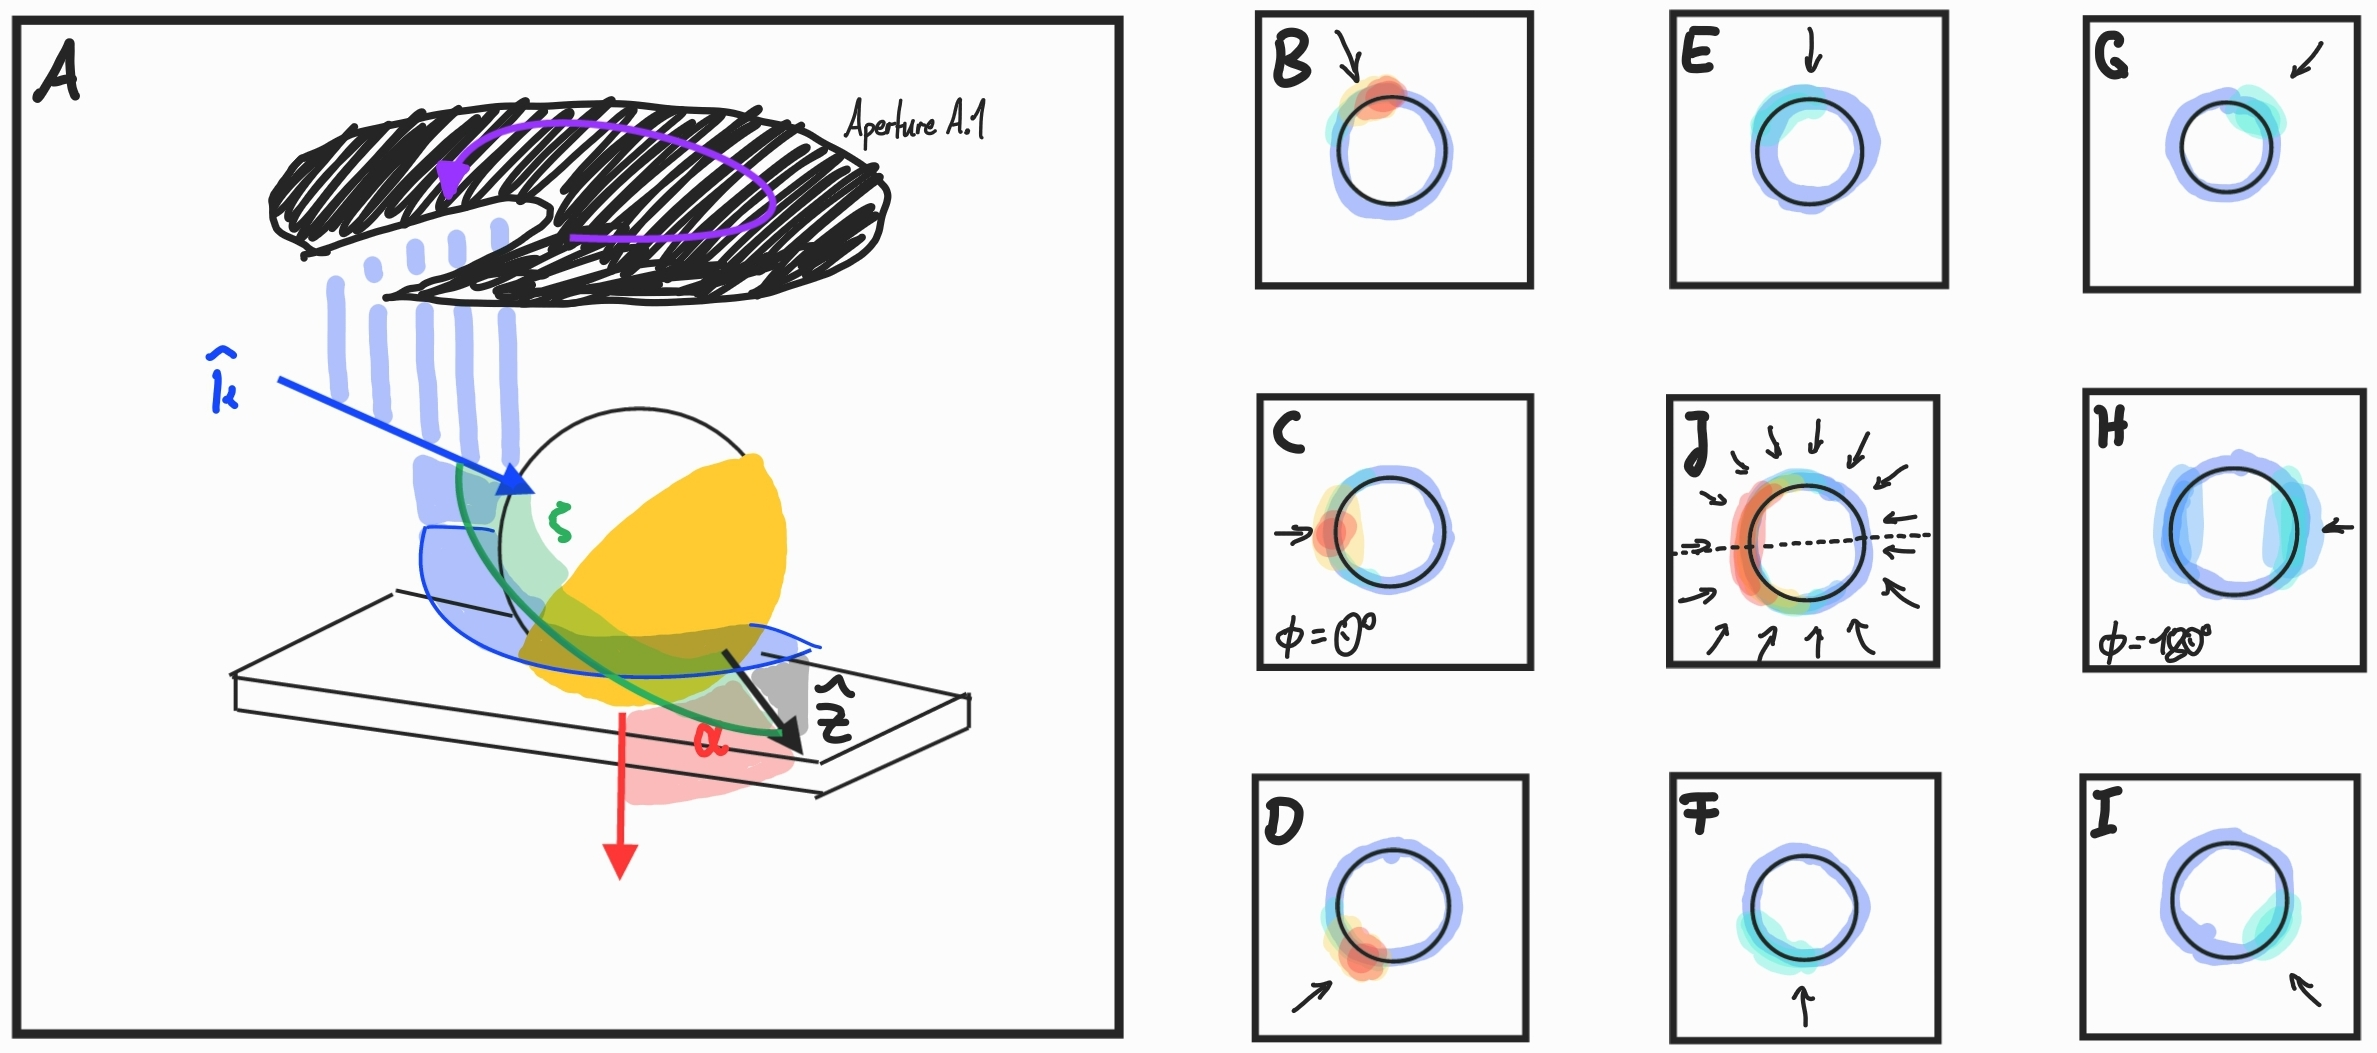
\includegraphics[width=\textwidth]{[fig] selective illumination}
    \caption{(Placeholder) Selective Illumination:   
    {\sffamily\bfseries A:} By rotating the aperture A.1 the direction of illumination on the particle can be controlled within the range permitted by its out-of-plane orientation. 
    {\sffamily\bfseries B-I:} Dark-field images of a JP under restricted illumination. 
    The arrows signify the in-plane angle of the illumination.  
    {\sffamily\bfseries J:} The same JP under unrestricted (normal) dark-field illumination. 
    }
    \label{fig:selective-illumination}
\end{figure*}
(Description of the procedure)

\subsection*{We find these results}
%We present spectra of scattered light from the JPs, resolved for different parameters.\\

The \textbf{sideways profiles} of the scattering intensity for a fixed wavelength produce something akin to \textbf{Mie plots}. 
\begin{figure*}[h!]
    \centering
    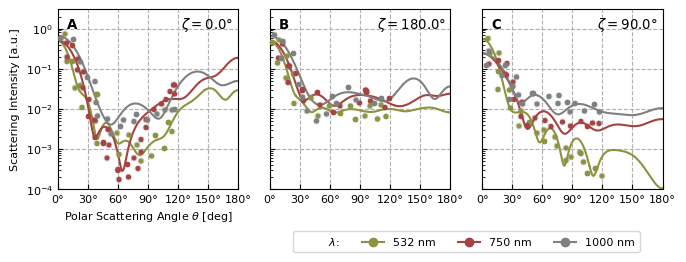
\includegraphics[width=\textwidth]{[fig] cartesian mieplots (3, placeholder)}
    \caption{Scattering intensity of the JP versus scattering angle. 
    The points signify measured intensities while the lines are simulation results.  
    {\sffamily\bfseries A} and {\sffamily\bfseries B} show the cylindrically symmetric cases of illumination from the PS side and from the Au side, respectively, i.e. where $\hat{k}\parallel\hat{z}$. 
    In {\sffamily\bfseries C}, the light is incident side-on ($\hat{k}\perp\hat{z}$, $\zeta=\pi/2$). 
    Disregarding the local extrema, qualitatively distinct large-scale behaviour is apparent: Under illumination from the PS side {\sffamily\bfseries (A)}, the scattering intensity becomes globally minimal in the sideways direction. 
    Meanwhile, under illumination from the Au side {\sffamily\bfseries (B)}, it reaches a plateau and under side-on illumination {\sffamily\bfseries (C)}, the scattering intensity drops consistently between forwards and backwards.  
    }
    \label{fig:jp-mieplots-oneline}
\end{figure*}

To our knowledge, this has never been done experimentally for individual particles. \\

%In general, most light is re-emitted in roughly the same direction that the illuminating light was propagating in. 
%If the particle is illuminated from the PS side, there is significantly more backward scattering and less sideways as compared to Au-side illumination. 
%Under side-on illumination, there is significantly less backward scattering than in either of the other cases. 
%Here, the small-scale peaks and valleys of the scattering intensity are much closer together. 
%This is similar to the shift from a smaller to a larger Mie-particle - when the illumination is incident from the side, the path length along which the light wave traverses the particle is longer (the diameter of the JP) than when the k-vector is in line with the particle's axis (in that case, it's the radius). \\

The large-scale shape of these Mie plots is appreciably different between the illumination direction. 
The small-scale shape (frequency of peaks and valleys) is also different for side-on versus Au-side or PS-side illumination. This, however is not resolved well in the experiment.\footnote{you can kind of see it, but you really need to squint your eyes}  \\

Even though the measurements can only show us an angular range of about 105° (because of the limited collection angle of the objective aperture), they match the simulation results well.\\


\begin{figure*}[h!]
    \centering
    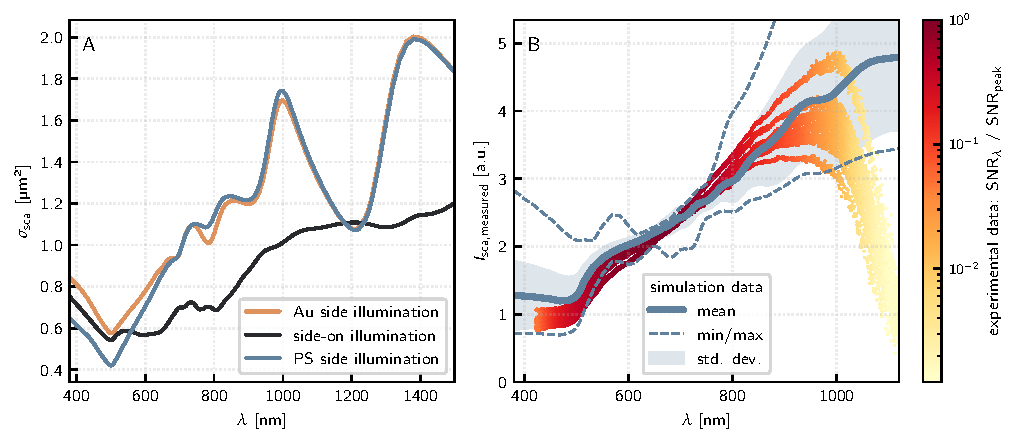
\includegraphics{[fig] spectra.PDF}
    \caption{{\sffamily\bfseries A:} simulated scattering spectrum of the JP under illumination from the Au side (yellow), from the PS side (blue) and from the equatorial side (black). {\sffamily\bfseries B:} measured scattering spectra (orange) atop value range as determined by simulation + emulation (blue).}
    \label{fig:spectra}
\end{figure*}

%One can also record a spectrum with an otherwise normal dark-field microscope. 
%Therein, the intensities are accumulated over all scattering angles within the collection range of the objective. 
%Moreover, the angles of illumination are also accumulated over the whole range that the out-of-plane angle of the particle and the NA of the dark-field condenser allow. 
%This accumulation can, of course, also be done with the simulation data. 
%They match. 



\subsection*{The Point}

We demonstrate a \textbf{versatile method} for the spectral analysis of optical scattering of plasmonic nanostructures. We apply this technique to plasmonic JPs, measuring scattering spectra with various orientation-dependencies. 

In addition, we complement these results with \textbf{numerical simulations}. Through the analysis of simulation data, we \textbf{correlate peaks} in the scattering spectra \textbf{to orientation-dependent surface plasmon modes}.

The experimental and numerical results match. 


\subsection*{Outlook}

The optical / visual detection of the out-of-plane angle of small JPs presents a problem. We expect that, based on our method, this can be done spectroscopically, in the future. \\




















\printbibliography














% Supplement starts here
\newpage


\section*{Supplementary Material}

\subsection*{Validation with Au NPs}

\begin{figure*}[h!]
    \centering
    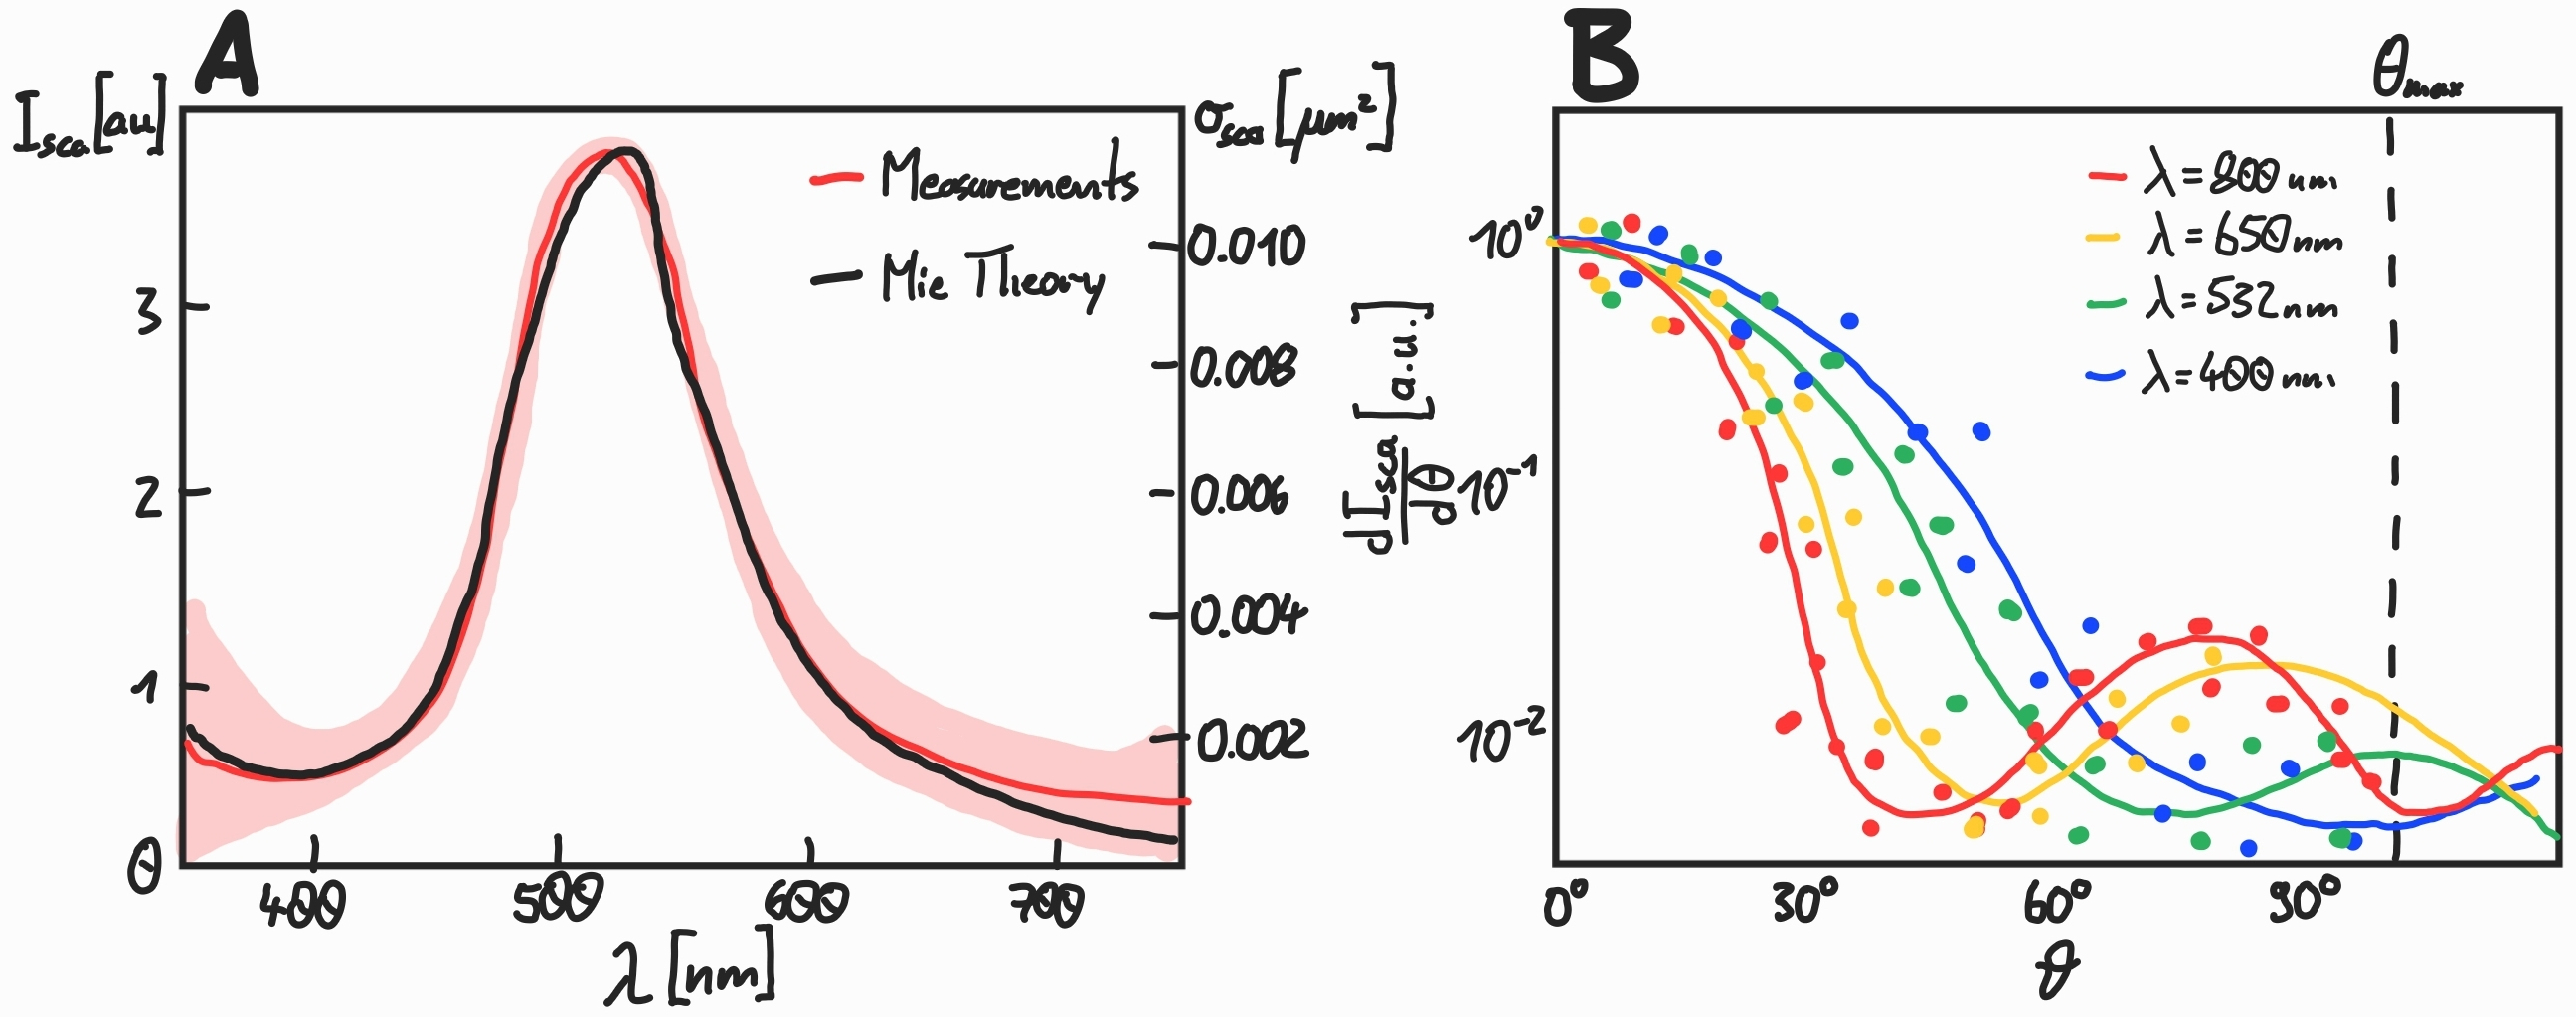
\includegraphics[width=\textwidth]{[fig] AuNP (placeholder).jpg}
    \caption{(Placeholder) 
    {\sffamily\bfseries A:} Scattering spectrum of 65 nm Au NPs. The shaded area corresponds to the SNR. 
    {\sffamily\bfseries B:} Scattering intensity of a spherical Au NP, $d=\SI{250}{\nano\meter}$ versus the scattering angle for various wavelengths. The lines show the predictions of GLMT \cite{GouesbetGrehan}, the points show measurement results.
    }
    \label{fig:AuNP}
\end{figure*}


\subsection*{Angular distributions for the JP, simulations only}

\begin{figure*}[h!]
    \centering
    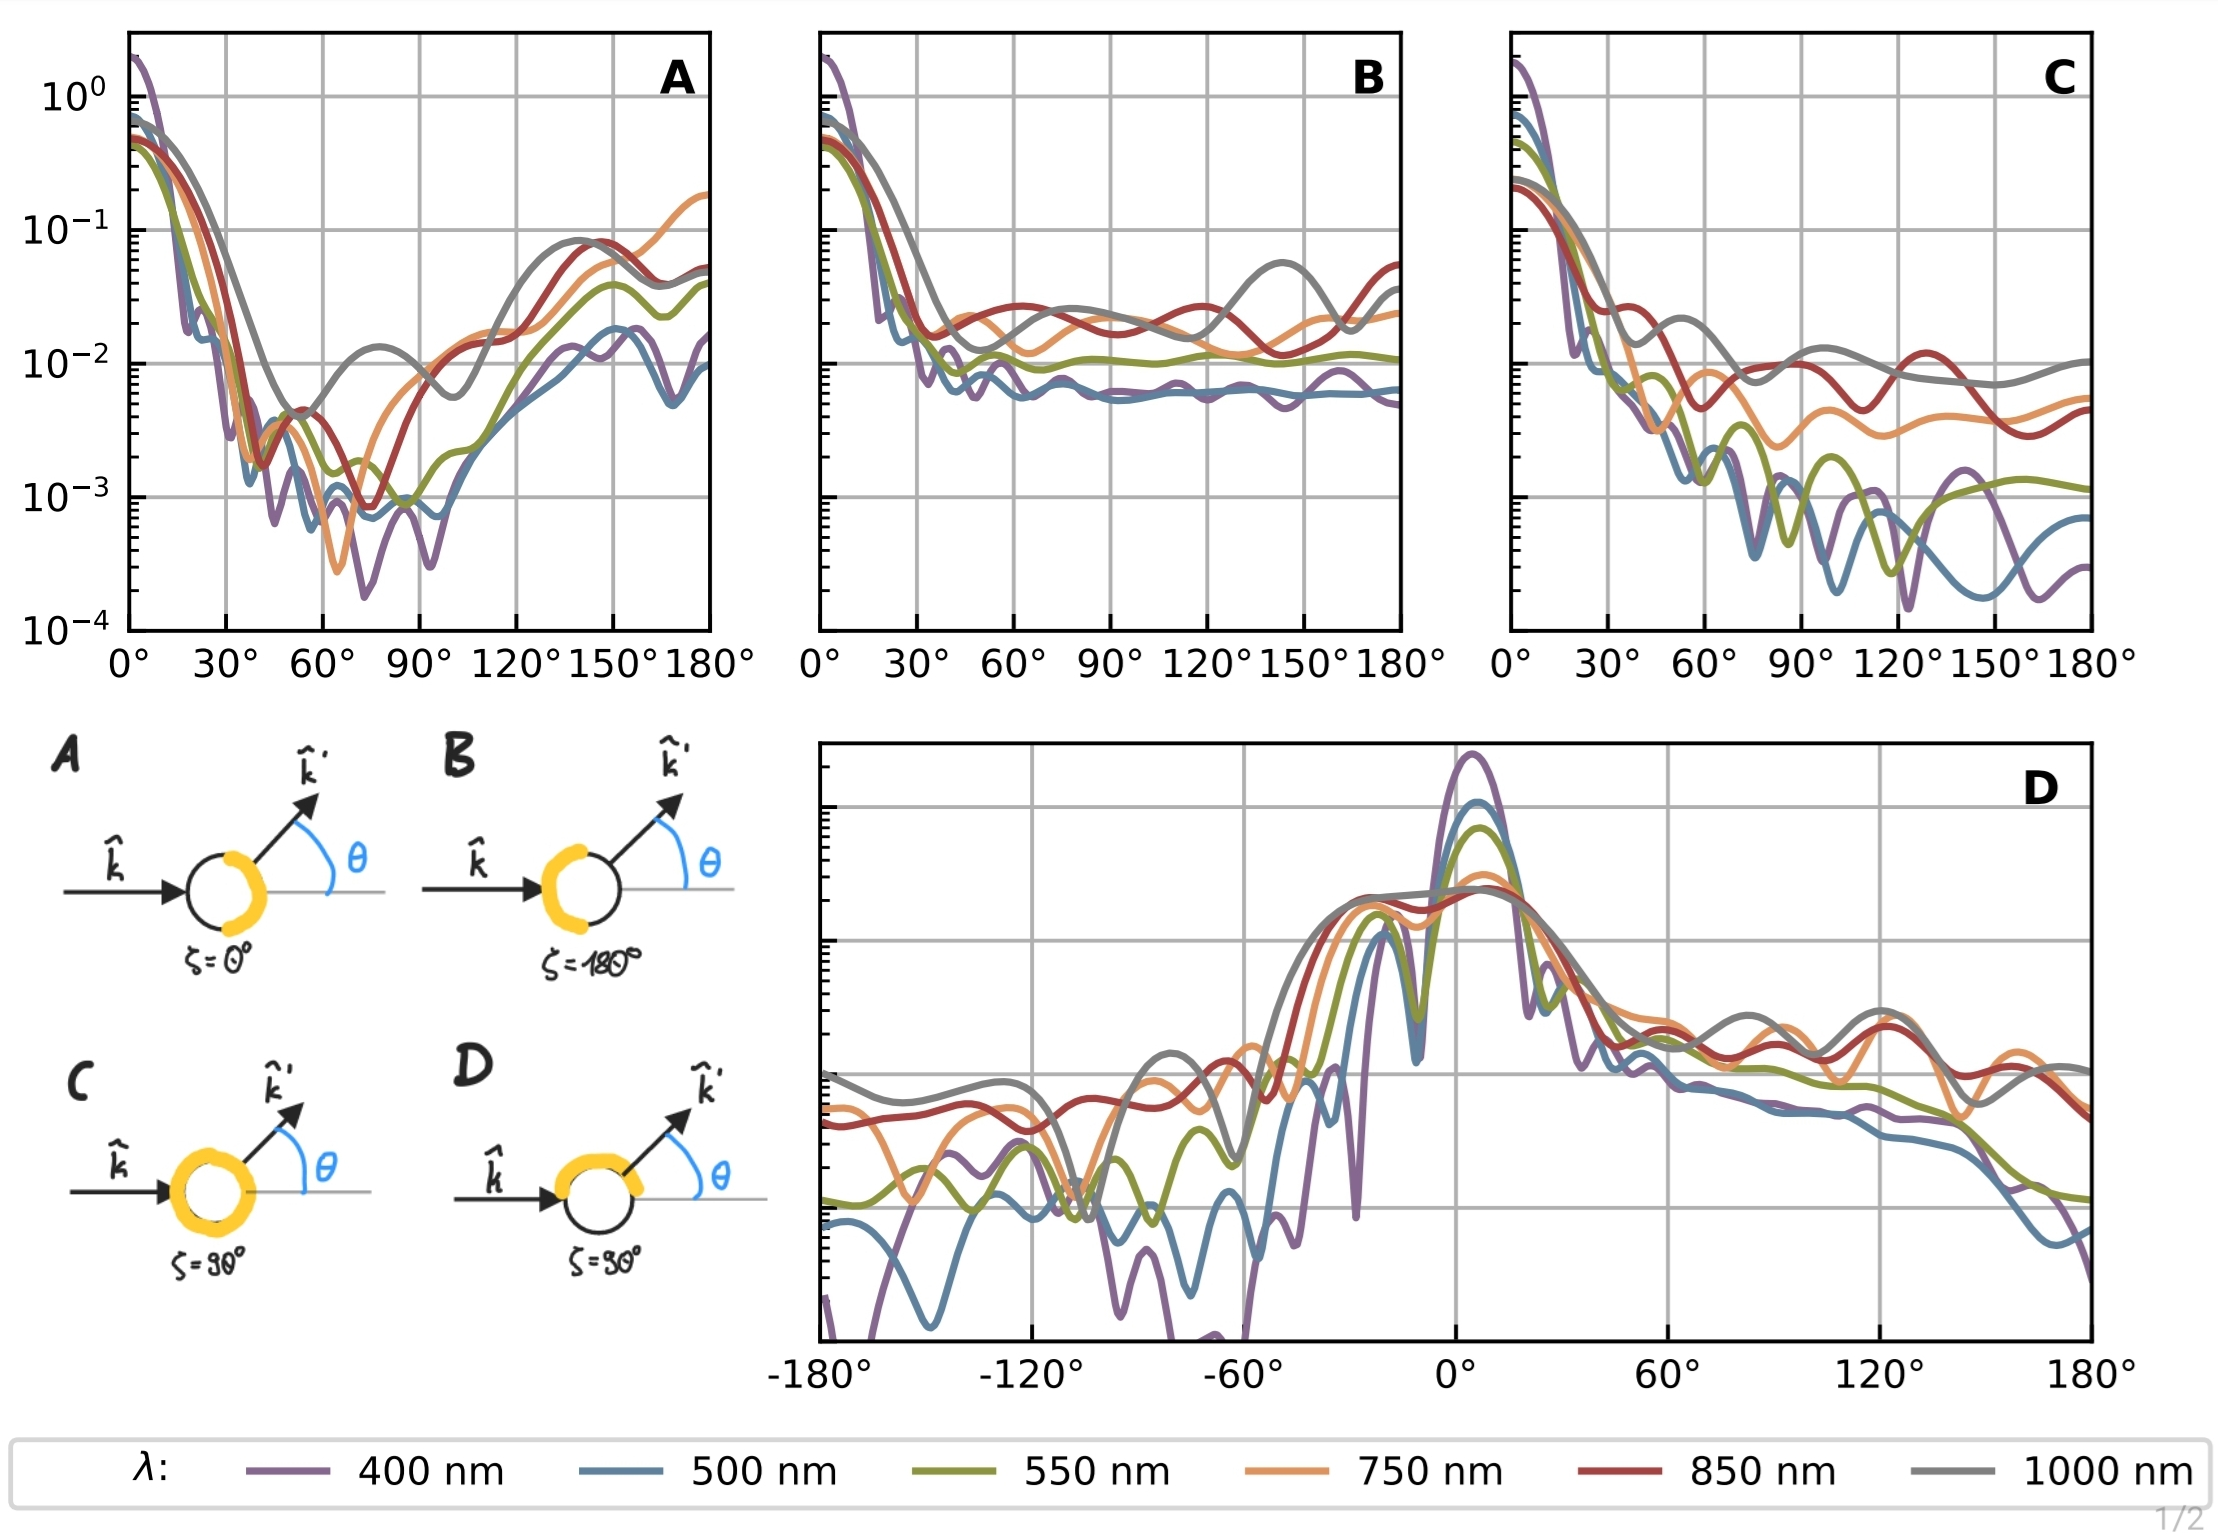
\includegraphics[width=\textwidth]{[fig] cartesian mieplots (placeholder).jpg}
    \caption{Scattering intensity of the JP versus scattering angle. 
    {\sffamily\bfseries A} and {\sffamily\bfseries B} show the cylindrically symmetric cases of illumination from the PS side and from the Au side, respectively, i.e. where $\hat{k}\parallel\hat{z}$. 
    In {\sffamily\bfseries C} and {\sffamily\bfseries D}, the light is incident side-on ($\hat{k}\perp\hat{z}$, $\zeta=\pi/2$).
    The scattering intensities are taken from the $(\hat{k},\hat{y})$ plane in {\sffamily\bfseries C} (note, that the system is still symmetric under inversion of $y$) and from the $(\hat{k},\hat{z})$ plane, where spatial symmetry is entirely broken, in {\sffamily\bfseries D}.
    Here, the Au side lies in the positive $\theta$ direction.  
    }
    \label{fig:jp-mieplots}
\end{figure*}


\end{document}
